\documentclass[12pt,a4paper]{article}
\synctex=1
\usepackage[utf8]{inputenc}
\usepackage[margin=1cm]{geometry}
\usepackage{graphicx}
%\usepackage{verbatim}
\usepackage{listings}
\usepackage{textcomp}
\usepackage{courier}
\usepackage{libertine}
\usepackage{pgfornament}
\usepackage{eso-pic}
\usepackage{amsmath}
\usepackage[hangul]{kotex}
\linespread{1.3}

\title{
	\centering
	\pgfornament[width=12cm,color=teal]{84}\\
	\vspace{1cm}
	\fontsize{50}{50} \selectfont {컴퓨터 그래픽스 입문}\\
		\pgfornament[width=12cm,color=teal]{88}\\
	\vfill}
\author{
	\LARGE
	\begin{tabular}{rl}
		\hline
		학번 : & 2016110056\\ 
		학과 : & 불교학부 \\
		이름 : & 박승원\\
		날짜 : & \today\\
		\hline
	\end{tabular}\vspace{2cm}
	\\

\includegraphics[width=0.5\textwidth]{logo.jpg}
	}
\date{}


\begin{document}
\maketitle
\pagenumbering{gobble}
\noindent
\lstset{language=C++, columns=flexible, tabsize=4, frame=shadowbox, showstringspaces=false, breaklines=true, upquote=true, basicstyle=\normalsize}
\newpage
\section*{Lab 13. 물리 엔진}
	
\begin{verbatim}
Problem 1. Use particle system to make a fountain similarly to the one
below: (5pts)
https://www.youtube.com/watch?v=rbS9_VzslFU

Problem 2. Implement damping to make your cloth simulation more stable. (5pts)\end{verbatim}
\section{분수}
\lstinputlisting[caption=fountain header]{src/fountain.h}
\lstinputlisting[caption=fountain implementation]{src/fountain.cc}
\lstinputlisting[caption=fountain main]{src/fountain.cpp}
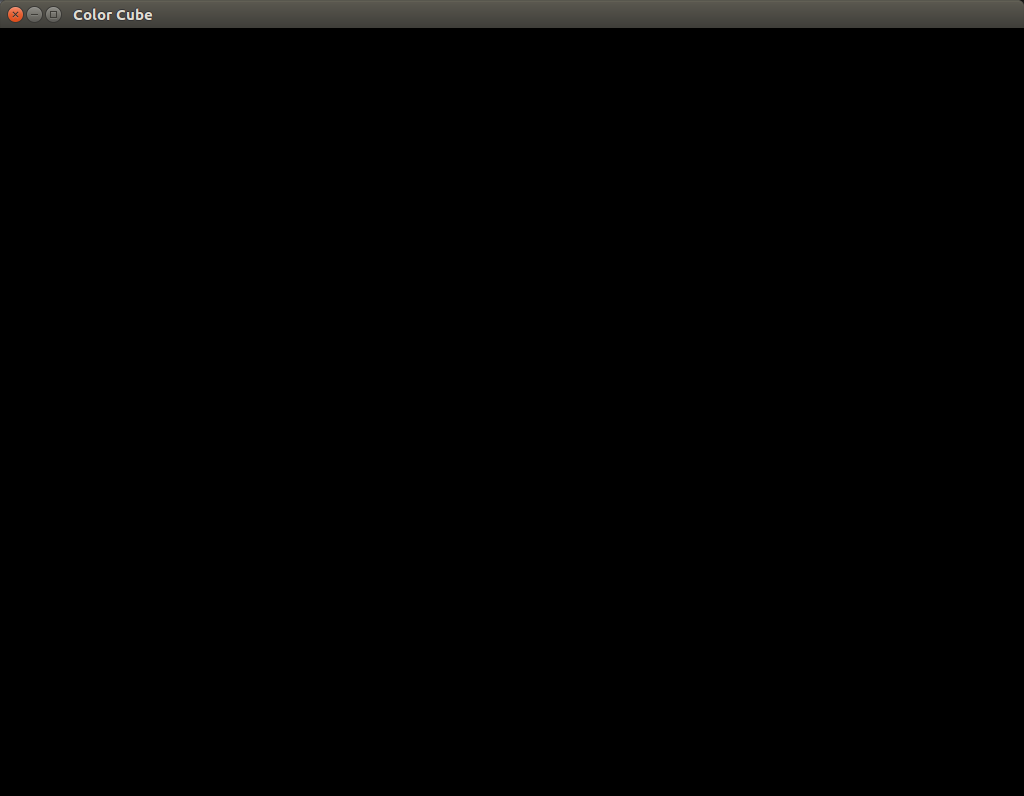
\includegraphics[width=0.7\textwidth]{2.png}

glEnable(GL\_PROGRMA\_POINT\_SIZE)한 후에 vertex shader에서 glPointSize를 설정해 준다.
그러나, 검은 화면만 나옴. 
버그가 있다.
2시간내에 물리엔진 두 개나 구현하기에는 조금 벅차다.
\section{커튼}
k=스프링상수, m=질량, x=위치, c=damping, x0=스프링이 달린 부분의 움직임,위치
\begin{gather*}
F = ma = -k(x-x_0) - c \frac{dx}{dt}\\
m\frac{d^2x}{dt^2} + c\frac{dx}{dt} + k(x - x_0) = 0\label{1}\tag{1}\\
let \quad \frac{dx}{dt} = z(t) \\
\frac{x(t + \Delta t)-x(t)}{\Delta t} = z(t)\\
x(t+\Delta t) = z(t)\Delta t + x(t) \tag{2}\\
from \eqref{1}\quad m\frac{dz}{dt} + cz(t) + k(x-x_0) = 0\\
m\frac{z(t+\Delta t)-z(t)}{\Delta t} + cz(t) + k(x-x_0)=0\\
z(t+\Delta t) = (cz(t) + k(x-x_0))\frac{\Delta t}{-m} +z(t)\tag{3}
\end{gather*}
위의 식 2,3으로부터 수치해석적으로 x(t)를 구할 수 있다.
\begin{lstlisting}
float SpringModel::time_pass(float x0, float dt) {
	x = z * dt + x;
	z = (c*z + k*(x - x0)) * dt / -m + z;
}
\end{lstlisting}
\lstinputlisting[caption=spring system header]{src/spring.h}
\lstinputlisting[caption=spring system implementation]{src/spring.cc}
\lstinputlisting[caption=main함수]{src/cloak.cpp}
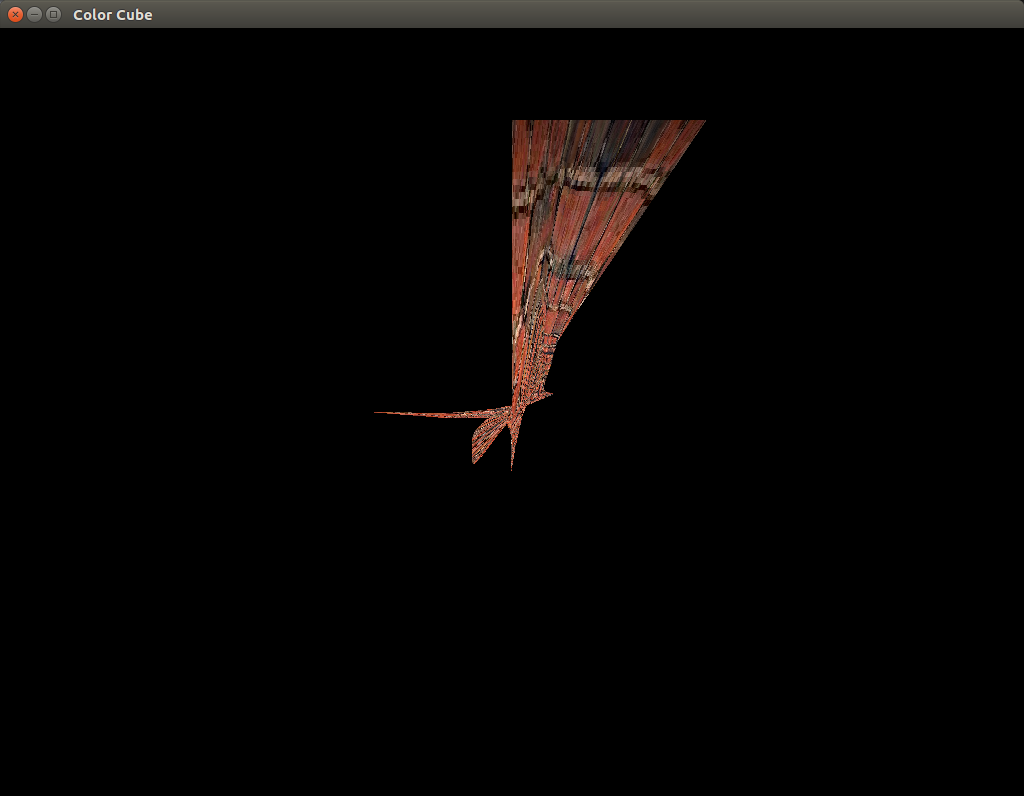
\includegraphics[width=0.7\textwidth]{1.png}

그냥 일차원에서 시험을 할 때는 괜찮았으나 삼차원으로 확장하는 과정에서 버그가 있다.
우선 중력 계산을 빠뜨렸다.
스프링 함수에 뭔가 버그가 있다. 
자연스러운 커튼이 되지 못하고 이상한 모양으로 움직인다.

\end{document}
